\subsection{Afinní prostor - $A_n$}
\begin{itemize}
	\item Je to prostor \textbf{obsahující body}. Navíc musí být současně dán \textbf{přidružený vektorový prostor} (souřadný systém) a nějaké \textbf{zobrazení}, které každé dvojici bodů přiřadí vektor (prvek z přidruženého vektorového prostoru).
	\item Cílem afinního prostoru je mít možnost \textbf{jednoznačně specifikovat body} pomocí jejich souřadnice a \textbf{manipulovat} s nimi s využitím prostředků lineární algebry.
	\item \textbf{Dimenze} vektorového prostoru určuje dimenzi afinního prostoru.
	\item Ukázka afinného prostoru:
	\begin{itemize}
		\item v trojrozměrném afinném prostoru $A_3$ máme bod $X$ se souřadnicemi $X=(x_1,x_2,x_3)$,
		\item vektor \textbf{x} je prvek onoho přidruženého vektorového prostoru.
	\end{itemize}
\end{itemize}


\subsubsection{Euklidovský prostor - $E_n$}
\begin{itemize}
	\item Afinní prostor ve kterém je zaveden \textbf{skalární součin}\eqref{skalar} a \textbf{norma}\eqref{norma} (velikost vektoru), to umožňuje měřit délku vektorů a úhly mezi nimi.
	\item Souřadný systém (kartézský, polární, válcový atd.).
\end{itemize}
\begin{equation}
\begin{split}
\label{skalar}
\textrm{Vektory }  a &= (a_1,a_2,a_3), \, b = (b_1,b_2,b_3) \\
 a \cdot b &= |a| \cdot |b| \cos \alpha, \\
 a \cdot b &= a_1b_1 + a_2b_2 +a_3b_3 \\ 
 \end{split}
\end{equation}
\begin{equation}
\label{norma}
 |a| = \sqrt{a_1^2 + a_2^2 + a_3^2} 
\end{equation}

\subsubsection{Kartézská souřadná soustava}
\begin{itemize}
	\item Souřadné osy jsou \textbf{vzájemně kolmé}.
	\item Protínají se v jednom bodě -- \textbf{počátku souřadná soustava}.
	\item Jednotka se obvykle volí na všech osách stejně velká.
	\item Souřadnice polohy bodu je možno dostat jako kolmé průměty polohy bodu k jednotlivým osám.
\end{itemize}

\subsection{Afinní transformace}
\begin{itemize}
	\item Afinní transformace je \textbf{zobrazení bodů jednoho afinního prostoru do jiného} afinního prostoru (speciální případ: zobrazení do téhož afinního prostoru (\textbf{bijekce}); tomu se říká afinita).
	\item Afinní transformace souřadnic je \textbf{geometrickou transformací} bodu $P=[x,y]$, jehož obrazem je bod $Q=[x',y']$, které spočívá v \textbf{posunutí} (translation), \textbf{otáčení} (rotation), \textbf{změně měřítka} (scaling), \textbf{zkosení} (shearing) nebo operaci \textbf{vzniklé jejim skládáním}.
	\item \textbf{Afinní} -- rovnoběžným přímkám odpovídají opět rovnoběžné přímky, které však nemusí být rovnoběžné s původními přímkami.
	\item Geometrické transformace jsou jedněmi z nejčastěji používaných operací v PG.
\end{itemize}
Když zavedeme následující vektory a matici:
\begin{equation*}
\begin{aligned}
 y = (y_1,y_2,y_3),  x = (x_1,x_2,x_3), t = (t_1,t_2,t_3),
 \end{aligned}
\end{equation*}
\begin{equation*}
 A = \begin{bmatrix}
     a_{11} & a_{12}  & a_{13}      \\[0.3em]
     a_{21} & a_{22}  & a_{23}      \\[0.3em]
     a_{31} & a_{32}  & a_{33} 
     \end{bmatrix}.
\end{equation*}
Můžeme \textbf{afinní transformaci} zapsat jako:
\begin{equation*}
 y = xA + t,
\end{equation*}
kde \textbf{y} je bod, do kterého je transformován bod \textbf{x} pomocí matice \textbf{A} a \textbf{translačního} vektoru \textbf{t}. Vektor \textbf{t} slouží k posunutí středu souřadné soustavy, matice \textbf{A} mění osy souřadné soustavy. Známe--li \textbf{A} a vektor \textbf{t}, můžeme transformaci jednoduše provést. Jindy se musí určit ze zadání.

\subsubsection{Ortonormalita afinní transformace}
\begin{itemize}
	\item Ortonormální transformace -- jsou takové transformace, které \textbf{nemění délky} ani \textbf{úhly}.
	\item Délky a úhly souvisejí se \textbf{skalárním součinem}, když se tento součin po transformaci \textbf{nezmění}, jsou zachovány délky i úhly.
	\item Vlastnosti ortonormální transformace:
		\begin{itemize}
			\item afinní transformace bude zachovávat hodnotu prévě tehdy, když $AA^T=I$, kde $I$ je jednotková matice (\textbf{nutná a postačující podmínka ortonormality}),
			\item také když uvážíme, že $A^{-1} = A^T$, pak platí $A^{-1} A^T = I$,
			\item determinant matice $\det(A)$ musí být roven $\pm 1$, protože $\det(AA^T) = \det(I)$ a $\det(I) = 1$.
			%co to je determinant here https://cs.wikipedia.org/wiki/Determinant
		\end{itemize}
\end{itemize}

\subsubsection{Afinní transformace (2D)}
\begin{itemize}
	\item \textbf{posunutí} (translation) -- posun ve směru x a y je dán hodnotou translačního vektoru,
	\begin{equation*}
 \begin{bmatrix}     
 x'   \\[0.3em]      
 y'
 \end{bmatrix} = 
 \begin{bmatrix}
     1 & 0     \\[0.3em]
     0 & 1        
  \end{bmatrix}
  \begin{bmatrix}
     x     \\[0.3em]
     y        
     \end{bmatrix} +
      \begin{bmatrix}
     b_x     \\[0.3em]
     b_y        
     \end{bmatrix}
\end{equation*}
	\item \textbf{otáčení} (rotation) -- ve směru ručiček (\textbf{naopak} prohodíš znaménka u $\sin$),
					\begin{equation*}
				 \begin{bmatrix}     
				 x'   \\[0.3em]      
				 y'
				 \end{bmatrix} = 
				 \begin{bmatrix}
				     \cos{\alpha} & -\sin{\alpha}     \\[0.3em]
				     \sin{\alpha} & \cos{\alpha}        
				  \end{bmatrix}
				  \begin{bmatrix}
				     x     \\[0.3em]
				     y        
				     \end{bmatrix} +
				      \begin{bmatrix}
				     0     \\[0.3em]
				     0        
				     \end{bmatrix}
					\end{equation*}
	\item \textbf{změna měřítka} (scaling),
				\begin{equation*}
			 \begin{bmatrix}     
			 x'   \\[0.3em]      
			 y'
			 \end{bmatrix} = 
			 \begin{bmatrix}
			     s_x & 0     \\[0.3em]
			     0 & s_y        
			  \end{bmatrix}
			  \begin{bmatrix}
			     x     \\[0.3em]
			     y        
			     \end{bmatrix} +
			      \begin{bmatrix}
			     0     \\[0.3em]
			     0        
			     \end{bmatrix}
				\end{equation*}
	\item \textbf{zkosení} (shearing),
				\begin{equation*}
			 \begin{bmatrix}     
			 x'   \\[0.3em]      
			 y'
			 \end{bmatrix} = 
			 \begin{bmatrix}
			     1 & sh_y     \\[0.3em]
			     sh_x & 1        
			  \end{bmatrix}
			  \begin{bmatrix}
			     x     \\[0.3em]
			     y        
			     \end{bmatrix} +
			      \begin{bmatrix}
			     0     \\[0.3em]
			     0        
			     \end{bmatrix}
				\end{equation*}
\end{itemize}

\subsubsection*{Skládání transformací (Příklad)}
Transformujte bod $A[3,4]$ posunem o vektor $(-5,1)$ a rotací o úhel $\ang{90}$ stupňů:
	\begin{equation*}
\textrm{posun:}
 \begin{bmatrix}     
 x'   \\[0.3em]      
 y'
 \end{bmatrix} = 
 \begin{bmatrix}
     1 & 0     \\[0.3em]
     0 & 1        
  \end{bmatrix}
  \begin{bmatrix}
     x     \\[0.3em]
     y        
     \end{bmatrix} +
      \begin{bmatrix}
     -5     \\[0.3em]
     1        
     \end{bmatrix} \qquad \textrm{rotace:}
	 \begin{bmatrix}     
	 x'   \\[0.3em]      
	 y'
	 \end{bmatrix} = 
	 \begin{bmatrix}
	     0 & -1     \\[0.3em]
	     1 & 0        
	  \end{bmatrix}
	  \begin{bmatrix}
	     x     \\[0.3em]
	     y        
	     \end{bmatrix} +
	      \begin{bmatrix}
	     0     \\[0.3em]
	     0        
	     \end{bmatrix}
\end{equation*}
\begin{figure}[H]
\centering
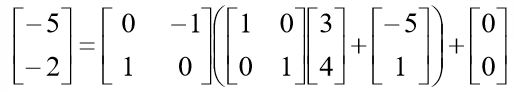
\includegraphics[width=0.7\textwidth]{assets/2_skladani}
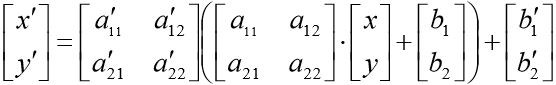
\includegraphics[width=0.7\textwidth]{assets/2_skladani2}
\end{figure}
\noindent Obecné \textbf{skládání transformací} v kartézské souřadné soustavě:
\begin{center}
$[X'] = A_n ...(A_2(A_1 \cdot X + b_1) + b_2) ... + b_n$.
\end{center}

\subsection{Projektivní prostor}
Při použití afinních prostorů v PG lze v některých situacích narazit na jisté problémy, zejména to, že nelze zobrazovat body v nekonečnu (tzv. nevlastní body). I když jsou praktické scény konečné, mohou i zde vzniknout \textbf{nevlastní body} (středové promítání). 

Problém spočívá v tom, že vektor reprezentovaný nevlastními body má jednu nebo více složek rovnou $\pm \infty$, kterou nelze v počítači jednoduše reprezentovat. Projektivní prostor navíc umožňuje promítání \textbf{středové} i \textbf{rovnoběžné} oproti prostoru afinnímu. Projektivní prostor tedy zavádí \textbf{homogenní souřadnice}, které jednotlivé body reprezentují.

\subsection{Homogenní souřadnice}
\begin{itemize}
	\item Myšlenkou je reprezentace bodu ve vektorovém prostoru o jednu dimenzi větší -- rozšíření o jednu dimenzi (expanze z 2D do 3D, popř. z 3D do 4D).
	\item Bod $(x,y)$ je v homogenních souřadnicích reprezentován jako $(wx,wy,w)$ kde $w \not= 0$.
	\item Nejčastěji volíme \textbf{homogenní souřadnici} $w = 1$.
	\item Bod se souřadnicemi $(x, y, w)$ má kartézské souřadnice $x' = x/w$ a $y' = y/w$. 
\end{itemize}
\begin{figure}[H]
\centering
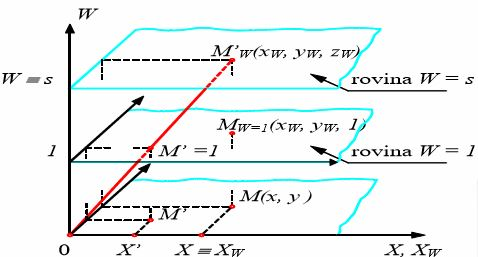
\includegraphics[width=0.7\textwidth]{assets/2_homoprostor}
\end{figure}

\subsection{Projektivní transformace - kolineace}
\begin{itemize}
	\item Kolineace je \textbf{zobrazení} bodů jednoho prostoru na body stejného nebo jiného prostoru.
	\item Kolineaci (projektivní transformaci) lze matematicky \textbf{popsat vztahem} $y = xT$, kde vektory $x$ a $y$ reprezentují před a po transformaci a matice $T$ charakterizuje \textbf{kolineaci} (transformační matice).
	\item Sehrává zásadní úlohu v grafických systémech, ty pracují nejčastěji s trojrozměrným projektivním prostorem, kde $T$ je ve tvaru  ve tvaru $4\times4$ a $x$, $y$ jsou čtyřprvkové vektory homogenních souřadnic.
\end{itemize}

\subsubsection{Základní transformace}
U projektivních transformací se můžeme setkat s těmito základními transformacemi:
\begin{itemize}
	\item \textbf{posunutí} (translation),
	\begin{equation*}
	T = \begin{bmatrix}
	1 & 0 & 0 & a      \\[0.3em]
	0 & 1 & 0 & b      \\[0.3em]
	0 & 0 & 1 & c      \\[0.3em]
	0 & 0 & 0 & 1      
	\end{bmatrix}
	\end{equation*}
	\item \textbf{otočení kolem osy x} (rotation),
	\begin{equation*}
	T = 	\begin{bmatrix}
	1 & 0 & 0 & 0        					\\[0.3em]
	0 & \cos{\theta} & -\sin{\theta} & 0    	\\[0.3em]
	0 & \sin{\theta} & \cos{\theta} & 0       \\[0.3em]
	0 & 0 & 0 & 1      
	\end{bmatrix}
	\end{equation*}
	\item \textbf{otočení kolem osy y} (rotation),
	\begin{equation*}
	T = 	\begin{bmatrix}
	\cos{\theta} & 0 & \sin{\theta} &  0      	\\[0.3em]
	0 & 1 & 0 & 0        						\\[0.3em]
	-\sin{\theta} & 0 & \cos{\theta} & 0       \\[0.3em]
	0 & 0 & 0 & 1      
	\end{bmatrix}
	\end{equation*}
	\item \textbf{otočení kolem osy z} (rotation),
	\begin{equation*}
	T = 	\begin{bmatrix}
	\cos{\theta} & \sin{\theta} & 0  & 0      	\\[0.3em]
	-\sin{\theta} & \cos{\theta} & 0 & 0       \\[0.3em]
	0 & 0 & 1 & 0        						\\[0.3em]
	0 & 0 & 0 & 1      
	\end{bmatrix}
	\end{equation*}
	\item \textbf{změna měřítka} (scaling),
	\begin{equation*}
	T = 	\begin{bmatrix}
	s_x & 0 & 0 & 0     	\\[0.3em]
	0 & s_y & 0 & 0      	\\[0.3em]
	0 & 0 & s_z & 0      	\\[0.3em]
	0 & 0 & 0 & 1      
	\end{bmatrix}
	\end{equation*}
	\item \textbf{zkosení} (shearing),
	\begin{equation*}
	T = 	\begin{bmatrix}
	1 & sh_y & 0 & 0       \\[0.3em]
	sh_x & 1 & 0 & 0       \\[0.3em]
	0 & 0 & 1 & 0       	\\[0.3em]
	0 & 0 & 0 & 1       
	\end{bmatrix}
	\end{equation*}
\end{itemize}

\subsection{Promítání}
\begin{itemize}
	\item \textbf{Promítání} -- zobrazení jednotlivých bodů na předem danou průmětnu.
	\item V geometrii nejprve volíme promítací metodu a potom v této zobrazujeme objekty (v PG naopak) -- nejprve vytvoříme objekt a následně volíme zobrazovací metodu vhodnou pro požadovaný účel.
	\item Definice promítání:
	\begin{itemize}
		\item \textbf{promítací paprsky} -- polopřímka, vycházející z promítacího bodu, směr závisí na typu promítání,
		\item \textbf{průmětna} (viewing plane) -- plocha v prostoru, na kterou dopadají promítací paprsky (paprsky vytvářející průmět),
		\item průmětnou nemusí být pouze rovina (polokoule, NURBS plocha...).
	\end{itemize}
\end{itemize}

\subsubsection{Klasifikace promítacích metod}
\begin{figure}[H]
\centering
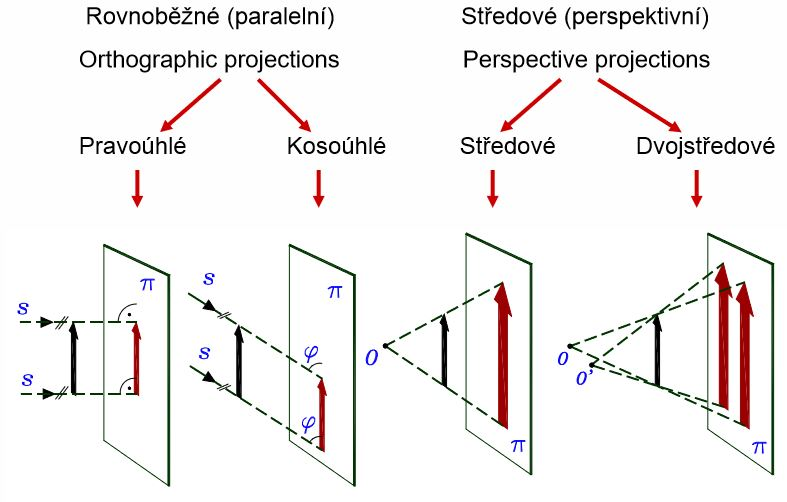
\includegraphics[width=0.7\textwidth]{assets/2_klas_promitani}
\end{figure}

\subsubsection{Rovnoběžné promítání}
Orthographic nebo orthogonal projection z řeckého \uv{orthos} rovný a \uv{graphe} kreslení. Promítání je určeno \textbf{průmětnou} \textbf{a} a směrem \textbf{s}, který není rovnoběžný s průmětnou.
\begin{equation*}
			 \begin{bmatrix}
			     1 & 0 & -\frac{d_x}{d_z} & 0       \\[0.3em]
    			 0 & 1 & -\frac{d_y}{d_z} & 0       \\[0.3em]
     			 0 & 0 & 1 & 0 	\\[0.3em]
     			 0 & 0 & 0 & 1       
			  \end{bmatrix}
		\end{equation*}
Matice popisuje rovnoběžné promítání na rovinu $xy$. Směr promítacího paprsku je $d = (d_x, d_y, d_z)$(viz obr).
\begin{figure}[H]
\centering
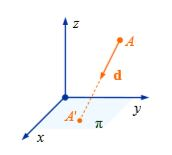
\includegraphics[width=0.3\textwidth]{assets/2_overeni_rovnobezneho_promitani}
\end{figure}
Jednička na pozici $3,3$ v matici zajišťuje, že se transformací nezmění souřadnice z bodu. Toho opět využívá řešení viditelnosti.
\subsection{Mongeova projekce}
\begin{itemize}
	\item Nejprve promítáme kolmo na vodorovnou rovinu $\pi$ (půdorysnu) -- promítací přímky jsou svislé, jde tedy o pohled shora (půdorys).
	\item Poté promítáme kolmo na svislo rovinu $v$ (nárysnu) -- promítací přímky jsou kolmé, jde tedy o pohled zpředu (nárys).
	\item Pohledy kreslíme bez přihlížení k obsahu sklopené druhé průmětny, tudíž se obrazy v jednotlivých průmětnách prolínají a jejich polohu v souřadnicovém systému popisuje vzdálenost od základnice (osa $Y$) potažmo od nulového bodu.
\end{itemize}
\begin{figure}[H]
\centering
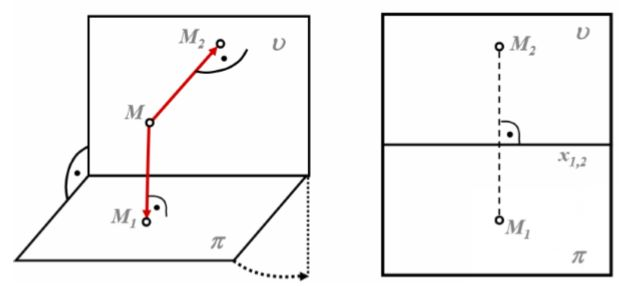
\includegraphics[width=0.6\textwidth]{assets/2_mongeova}
\end{figure}

Souřadnice bodů: $M(x, y, z)$... 1. průmět $M1 (x, y, 0)$ 2. průmět $M2 (x, 0, z)$. V Mongeově projekci je\textbf{ těleso určeno svým nárysem a půdorysem}.
\subsection{Kosoúhlé promítání}
\begin{itemize}
	\item Je rovnoběžné promítání na jednu průmětnu směrem, který má odchulku $\varphi$ jinou než \ang{90} od průmětny, promítací paprsky $S$ jsou tak rovnoběžné a ne kolmé k průmětně $\pi$. Průmětna $\pi$ je rovnoběžná s některou hlavních rovin.
	\item \textbf{Výhodou} tohoto způsobu je skutečnost, že \textbf{předměty}, které se nacházejí v nárysně \textbf{jsou zobrazeny v reálné velikosti}.
\end{itemize}
\subsection{Axonometrie - rovnoběžné, pravoúhlé promítání}
\begin{itemize}
	\item Axonometrie nebo axonometrické projekce je jednoduchý způsob promítání prostorových těles a trojrozměrných struktur do roviny.
	\item V rovině se nejprve zvolí tři osy $x, y, z$, jež spolu svírají stejné nebo nestejné úhly.
	\item Rozměry těles se pak nanášejí v určitém měřítku rovnoběžně s těmito osami.
	\item Hlavní výhoda axonometrie proti složitějším metodám promítáné je v tom, že průmět se snadno konstruuje, a že se z něho dají rozměry odečíst.
	\item Nevýhoda může být v tom, že v axonometrické projekci se rovnoběžky nesbíhají a tak je perspektivní dojem nedokonalý (může působit vizuální paradox).
\end{itemize}

\begin{figure}[H]
\centering
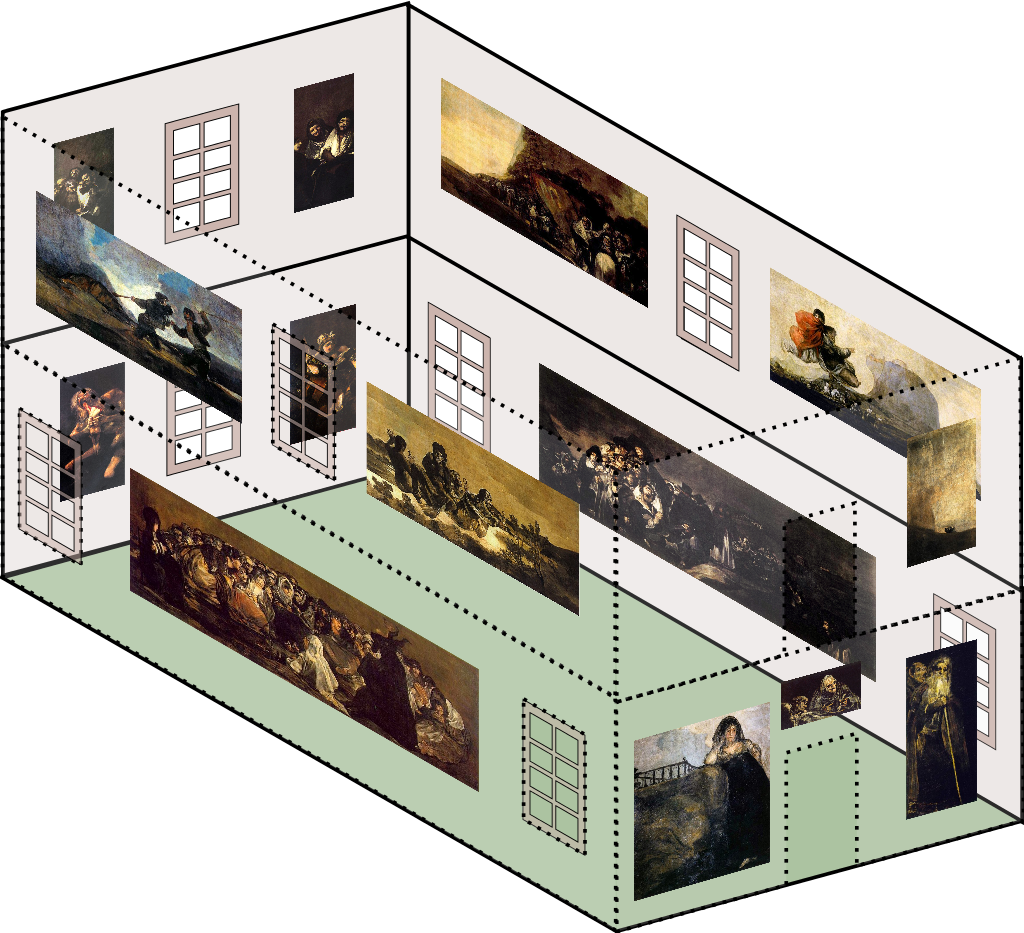
\includegraphics[width=0.3\textwidth]{assets/2_axonometrie}
\end{figure}

\subsection{Ortogonální promítání}
\begin{itemize}
	\item Směr promítání kolmý k průmětně (jedná se tedy o speciální případ rovnoběžného promítání).
	\item Zachovávají se všechny vlastnosti rovnoběžného promítání.
\end{itemize}
\begin{figure}[H]
\centering
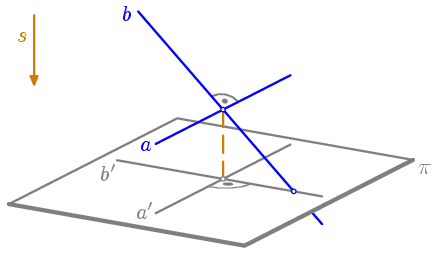
\includegraphics[width=0.4\textwidth]{assets/2_ortogonalni.png}
\end{figure}
\subsection{Perspektiva -- středové promítání}
\begin{equation*}
			 \begin{bmatrix}
			     1 & 0 & 0 & 0       \\[0.3em]
    			 0 & 1 & 0 & 0       \\[0.3em]
     			 0 & 0 & 1 & \frac{-1}{f} 	\\[0.3em]
     			 0 & 0 &  0 & 1       
			  \end{bmatrix}
		\end{equation*}
Matice popisuje projekci ze středu o souřadnicích $(0, 0, f)$ na rovinu $z = 0$ (tedy na rovinu  $xy$).
\begin{figure}[H]
\centering
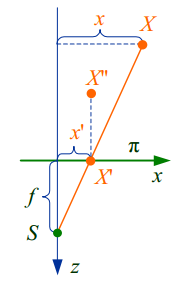
\includegraphics[width=0.2\textwidth]{assets/2_stredove_promitani}
\end{figure}
Ačkoliv se očekává, že po transformaci bodu bude jeho z souřadnice rovna $0$, není to pravda. Tuto nenulovou hodnotu však lze využít například při řešení viditelnosti. Souřadnice $x$ a $y$ slouží k vykreslení na obrazovku.
\subsection{Modelovací transformace}
Jsou všechny transformace, pomocí nichž se \textbf{vytváří scéna}: posun, zkosení, rotace, změna velikosti.

\subsection{Zobrazovací transformace}
Transformace používané k \textbf{zobrazení scény}: středové a rovnoběžné zobrazení. Jsou dělány tak, aby výsledky padly do jednotkového zobrazovacího objemu - souřadnice z intervalu $\langle -1, 1 \rangle$. 